\chapter{Simulations}
\label{ch:results}
In this chapter we get to test our implementation.

We evaluate the reconstruction performance, we use the relative reconstruction error and the peak signal-to-noise ratio.
We conduct four experiments in which we aim to compare the performance under different scenarios.

To close off with, we show some examples.

\section{Performance Metrics}
In this section, we will introduce three performance metrics that are often used to measure the quality of reconstructed images and videos.

Let $\bm{\hat v} \in\mathbb{R}^M$ be a reconstructed signal (in vectorized form) and let $\bm v$ be the corresponding orginal signal.
The \emph{mean square error} (MSE) of the reconstruction is defined as
\begin{equation*}
  \mse(\bm{\hat v}) = \frac{\sum_{i=1}^M (\hat v_i - v_i)^2}{M}
\end{equation*}
The MSE is zero if and only if we $\bm{\hat v}$ is an exact reconstruction of $\bm v$.

Using the MSE, we can compute the \emph{Peak Signal-to-Noise Ratio} (PSNR) of the reconstruction:
\begin{equation*}
  \psnr(\bm{\hat v}) = 10 \cdot \log_{10} \left(\frac{R^2}{\mse(\bm{\hat v})}\right)
\end{equation*}
where $R$ is the maximum fluctuation in the input signal data type. 
For grayscale images or videos in which the pixel values are stored as 8-bit unsigned integers, we have that $R = 256$.

The PSNR is usually expressed in term of decibel (dB). 
Higher values of the PSNR correspond to more accurate reconstructions.
The PSNR is widely used in the image and video compression literature to measure the quality of a compressed signal.
Generally, when comparing the reconstruction quality, the PSNR should only be used if it was measured on the same signal.

The final performance metric that we compute is the \emph{relative reconstruction error}.
It is given by
\begin{equation*}
  \rre(\bm{\hat v}) = \frac{||\bm{\hat v} - \bm v||_2}{||\bm v||_2}
\end{equation*}
This is the metric that was used in \cite{ji2008} and \cite{pilikos2014}.

\section{Experiments}
Four experiments were conducted that show what sort of performance one can expect under different settings.
All simulations were run using the ``foreman'' test video.

For each experiment, we plot the performance against the number of CS measurements as a percentage of the signal size.
Two plots are generated per experiment, one using the RRE and the other using the PSNR as performance measure.

Throughout the simulations, the block size is kept constant at $8\times 8\times 8$.

\subsection{MSCE vs BCS}
The results of the first experiment are shown in Figure \ref{fig:sim_msce}.
In the first experiment, we compare the performance of the MSCE algorithm to the BCS algorithm in the problem of video interpolation.

We run 3 instances of the BCS algorithm using Haar wavelet basis at scales 1, 2 and 3, respectively.
We see that when the number of CS measurements $N$ is small compared to the size of the signal $M$, a BCS using Haar wavelets at scale 1 performs very poorly.
As $N$ increases, its performance begins to accelarate and for $N > 0.5M$, the scale 1 Haar basis functions outperform the Haar bases at scales 2 and 3. 

We should expect this behaviour from our analysis in Section \ref{sect:interpol_haar}.
At low measurement rates, the BCS with level 1 Haar wavelets is unable to fill in the entire signal.
However, at the portions of the signal where the reconstruction succeeds, it will generally be of higher quality than that of the BCS using wavelets at higher scales.

Next, we run the MSCE algorithm with 3 cascades.
We can see immediately that a cascade of BCS algorithms is superior to any individual BCS instance that uses Haar wavelets.

The performances of the MSCE and the BCS using level 1 wavelets converge as the number of measurements $M$ increases.
That is because, for large $M$, the later stages of the cascade become redundant as Haar wavelets at scale 1 manage to cover any missing signal values.

Finally, we also run an instance of the BCS algorithm that uses DCT basis functions.
We see that it easily outperforms even the cascade.
Only in extremely undersampled situations ($N<0.2M$) does the MSCE have an advantage over the BCS with DCT basis functions.

A possible explanation is that the sparsifying properties of the DCT are superior to those of the Haar wavelet DWT.
Haar wavelets are the simplest of all wavelet functions.
It would be interesting to compare these performances to that of a MSCE which uses more sophisticated wavelet functions, such as the CDF 9/7 wavelets.

%% CASCADE
\begin{figure}
  \centering
  \begin{tikzpicture}[scale = 0.8,baseline]
    \begin{axis}[
      xlabel=$N/M$ (\%),
      ylabel=$\rre$ (\%),
      xmin=0, xmax = 100,
      ymin = 0, ymax = 0.2,
      scaled ticks=false,
      legend style={
        at={(0.99,1.1)},
        anchor=north east,
      },
      smooth,
      yticklabel style={
        /pgf/number format/precision=2,
        /pgf/number format/fixed,
      }
      ]
      \addplot table [x=pc, y=rre] {Chapter7/Images/MSCE.dat};      
      \addlegendentry{MSCE}
      \addplot table [x=pc, y=rre] {Chapter7/Images/MASK_3.dat};      
      \addlegendentry{BCS Scale 3}
      \addplot table [x=pc, y=rre] {Chapter7/Images/MASK_2.dat};     
      \addlegendentry{BCS Scale 2}
      \addplot table [x=pc, y=rre] {Chapter7/Images/MASK_1.dat};
      \addlegendentry{BCS Scale 1}
      \addplot[olive,mark=diamond*] table [x=pc, y=rre] {Chapter7/Images/DCT.dat};
      \addlegendentry{BCS DCT}
    \end{axis}
  \end{tikzpicture}
  % 
  \hskip 10pt
  % 
  \begin{tikzpicture}[scale = 0.8,baseline]
    \begin{axis}[
      xlabel=$N/M$ (\%),
      ylabel=$\psnr$ (dB),
      xmin=0, xmax = 90, 
      scaled ticks=false,
      legend style={
        at={(0.01,1.1)},
        anchor=north west,
      },
      yticklabel style={
        /pgf/number format/precision=2,
        /pgf/number format/fixed,
      },
      ylabel style={at={(1.4,0.5)}, anchor=south},
      yticklabel pos=right,      
      minor y tick num = 1,
      ]
      \addplot table [x=pc, y=psnr] {Chapter7/Images/MSCE.dat};      
      \addlegendentry{MSCE}
      \addplot table [x=pc, y=psnr] {Chapter7/Images/MASK_3.dat};
      \addlegendentry{BCS Scale 3}
      \addplot table [x=pc, y=psnr] {Chapter7/Images/MASK_2.dat};
      \addlegendentry{BCS Scale 2}
      \addplot table [x=pc, y=psnr] {Chapter7/Images/MASK_1.dat};
      \addlegendentry{BCS Scale 1}
      \addplot[olive,mark=diamond*] table [x=pc, y=psnr] {Chapter7/Images/DCT.dat};
      \addlegendentry{BCS DCT}
    \end{axis}
  \end{tikzpicture}
\caption{Performance of MSCE with 3 cascades and uniform Masks}
\label{fig:sim_msce}
\end{figure}

\subsection{DCT vs Haar with Gaussian \texorpdfstring{$\bm\Theta$}{[Theta]}}
In the second experiment we compare the performance of DCT and Haar basis functions in the case when $\bm\Theta$ consists of Gaussian samples.

We simulate Compressive Sensing measurements that were acquired via a random Gaussian sensing mechanism $\bm\Theta$.

The reconstruction quality of the BCS with DCT basis functions and the BCS with level 3 Haar basis functions is shown Figure \ref{fig:sim_basis}.
In this case, we see that the DCT outperforms the Haar basis function at all compression levels.

%% BASIS
\begin{figure}
  \centering
  \begin{tikzpicture}[scale = 0.8,baseline]
    \begin{axis}[
      xlabel=$N/M$ (\%),
      ylabel=$\rre$ (\%),
      xmin=0, xmax = 100,
      ymin = 0,
      smooth, 
      scaled ticks=false,
      yticklabel style={
        /pgf/number format/precision=2,
        /pgf/number format/fixed,
      }
      ]
      \addplot table [x=pc, y=rre] {Chapter7/Images/GAUSS_DCT.dat};      
      \addlegendentry{DCT}
      \addplot table [x=pc, y=rre] {Chapter7/Images/GAUSS_HAAR.dat};      
      \addlegendentry{Haar}
    \end{axis}
  \end{tikzpicture}
  % 
  \hskip 10pt
  % 
  \begin{tikzpicture}[scale = 0.8,baseline]
    \begin{axis}[
      xlabel=$N/M$ (\%),
      ylabel=$\psnr$ (dB),
      xmin=0, xmax = 90,      
      scaled ticks=false,
      legend style={
        at={(0.03,0.98)},
        anchor=north west,
      },
      smooth,
      yticklabel style={
        /pgf/number format/precision=2,
        /pgf/number format/fixed,
      },
      ylabel style={at={(1.4,0.5)}, anchor=south},
      yticklabel pos=right,      
      ]
      \addplot table [x=pc, y=psnr] {Chapter7/Images/GAUSS_DCT.dat};      
      \addlegendentry{DCT}
      \addplot table [x=pc, y=psnr] {Chapter7/Images/GAUSS_HAAR.dat};      
      \addlegendentry{Haar}
    \end{axis}
  \end{tikzpicture}
\caption{DCT vs Haar DWT (scale 3) with Gaussian measurements}
\label{fig:sim_basis}
\end{figure}


\subsection{Gaussian vs Bernoulli vs Random Signal Masks}
The aim of the third experiment is to see how reconstruction differs if we change the sensing mechanism.

We simulate three sets of CS measurements using Gaussian, Bernoulli and random signal mask sensing matrices.
The reconstruction is done using via the BCS algorithm and uses DCT basis functions.

Figure \ref{fig:sim_sensor} shows the result of that experiment.
We get near-identical performance in all three scenarios.

Only when the number of measurements is relatively high ($N\geq 0.8M$) do we begin to see a slight difference in the reconstruction quality.

%% SENSORS
\begin{figure}
  \centering
  \begin{tikzpicture}[scale = 0.8,baseline]
    \begin{axis}[
      xlabel=$N/M$ (\%),
      ylabel=$\rre$ (\%),
      xmin=0, xmax = 100,
      ymin = 0, 
      scaled ticks=false,
      yticklabel style={
        /pgf/number format/precision=2,
        /pgf/number format/fixed,
      },
      smooth,
      ]
      \addplot table [x=pc, y=rre] {Chapter7/Images/GAUSS_DCT.dat};      
      \addlegendentry{Gauss}
      \addplot table [x=pc, y=rre] {Chapter7/Images/BERN_DCT.dat};      
      \addlegendentry{Bernoulli}
      \addplot table [x=pc, y=rre] {Chapter7/Images/MASK_DCT.dat};      
      \addlegendentry{Mask}
    \end{axis}
  \end{tikzpicture}
  % 
  \hskip 10pt
  % 
  \begin{tikzpicture}[scale = 0.8,baseline]
    \begin{axis}[
      xlabel=$N/M$ (\%),
      ylabel=$\psnr$ (dB),
      xmin=0, xmax = 90,      
      scaled ticks=false,
      legend style={
        at={(0.03,0.98)},
        anchor=north west,
      },
      smooth,
      yticklabel style={
        /pgf/number format/precision=2,
        /pgf/number format/fixed,
      },
      ylabel style={at={(1.4,0.5)}, anchor=south},
      yticklabel pos=right,      
      ]
      \addplot table [x=pc, y=psnr] {Chapter7/Images/GAUSS_DCT.dat};      
      \addlegendentry{Gauss}
      \addplot table [x=pc, y=psnr] {Chapter7/Images/BERN_DCT.dat};      
      \addlegendentry{Bernoulli}
      \addplot table [x=pc, y=psnr] {Chapter7/Images/MASK_DCT.dat};      
      \addlegendentry{Mask}
    \end{axis}
  \end{tikzpicture}
\caption{Gaussian vs Bernoulli vs Mask (uniform) with DCT basis}
\label{fig:sim_sensor}
\end{figure}

% \subsection{Comparison of different Scales of Haar Wavelets when \texorpdfstring{$\bm\Theta$}{[Theta]} is Gaussian}
% In the first experiment, we saw that Haar wavelets at scale 1 give bad performance at high compression levels.
% However, if the number of measurements is sufficiently high, they will outperform Haar wavelets at higher scales, due to their localized support.

% However, if $\bm\Theta$ is a random matrix of Gaussian samples, then the discussion in Section \ref{sect:interpol_haar} no longer applies.

% Thus, we expect there to no 
% We saw that, when $\bm\Theta$ is a signal mask and we wish to perform the reconstruction using Haar wavelets,

% %% SCALES
% \begin{figure}
%   \centering
%   \begin{tikzpicture}[scale = 0.8,baseline]
%     \begin{axis}[
%       xlabel=$N/M$ (\%),
%       ylabel=$\rre$ (\%),
%       xmin=0, xmax = 100,
%       ymin = 0,
%       smooth, 
%       scaled ticks=false,
%       yticklabel style={
%         /pgf/number format/precision=2,
%         /pgf/number format/fixed,
%       }
%       ]
%       \addplot table [x=pc, y=rre] {Chapter7/Images/HAAR_GAUSS_1.dat};      
%       \addlegendentry{Scale 1}
%       \addplot table [x=pc, y=rre] {Chapter7/Images/HAAR_GAUSS_2.dat};
%       \addlegendentry{Scale 2}
%       \addplot table [x=pc, y=rre] {Chapter7/Images/HAAR_GAUSS_3.dat};
%       \addlegendentry{Scale 3}
%     \end{axis}
%   \end{tikzpicture}
%   % 
%   \hskip 10pt
%   % 
%   \begin{tikzpicture}[scale = 0.8,baseline]
%     \begin{axis}[
%       xlabel=$N/M$ (\%),
%       ylabel=$\psnr$ (dB),
%       xmin=0, xmax = 90,      
%       scaled ticks=false,
%       legend style={
%         at={(0.03,0.98)},
%         anchor=north west,
%       },
%      smooth,
%       yticklabel style={
%         /pgf/number format/precision=2,
%         /pgf/number format/fixed,
%       },
%       minor y tick num = 1,
%       ylabel style={at={(1.4,0.5)}, anchor=south},
%       yticklabel pos=right,      
%       ]
%       \addplot table [x=pc, y=psnr] {Chapter7/Images/HAAR_GAUSS_1.dat};
%       \addlegendentry{Scale 1}
%       \addplot table [x=pc, y=psnr] {Chapter7/Images/HAAR_GAUSS_2.dat};
%       \addlegendentry{Scale 2}
%       \addplot table [x=pc, y=psnr] {Chapter7/Images/HAAR_GAUSS_3.dat};
%       \addlegendentry{Scale 3}
%     \end{axis}
%   \end{tikzpicture}
% \caption{Haar wavelets at different scales with Gaussian measurements (fixed block size)}
% \label{fig:sim_scales}
% \end{figure}

\clearpage

\section{Example Results}


% \begin{figure}
%   \centering
%   \textbf{\hspace{0.2in} Frame 32 \hspace{1.5in} Frame 52\hspace{0.5in}\vspace{0.1in}}
%   \begin{subfigure}{0.4\textwidth}
%     \centering
%     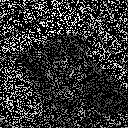
\includegraphics[width=0.9\textwidth]{Chapter7/Images/foreman_haar_masked_64.png}
%     \caption{Corrupted}
%   \end{subfigure}
%   \begin{subfigure}{0.4\textwidth}
%     \centering
%     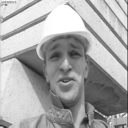
\includegraphics[width=0.9\textwidth]{Chapter7/Images/foreman_haar_orig_64.png}
%     \caption{Corrupted}
%   \end{subfigure}
%   \begin{subfigure}{0.4\textwidth}
%     \centering
%     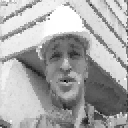
\includegraphics[width=.9\textwidth]{Chapter7/Images/foreman_haar_rec_64.png}
%     \caption{Recovered}
%   \end{subfigure}
%   \begin{subfigure}{0.4\textwidth}
%     \centering
%     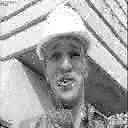
\includegraphics[width=.9\textwidth]{Chapter7/Images/foreman_dct_rec_64.png}
%     \caption{Recovered}
%   \end{subfigure}
%   \caption{Reconstruction of $128\times 128\times 128$ video signal ``akiyo'' from 70\% of the measurement using the MSCE with 3 cascades. Mask decimation pattern is uniform. $\psnr = 36.86$}
% \end{figure}

\begin{figure}[!ht]
  \centering
  \textbf{\hspace{0.2in} Frame 2 \hspace{1.5in} Frame 19\hspace{0.5in}\vspace{0.2in}}
  \begin{subfigure}{0.4\textwidth}
    \centering
    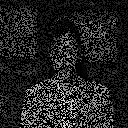
\includegraphics[width=0.8\textwidth]{Chapter7/Images/akiyo40_masked_2.png}
    \caption{Corrupted}
  \end{subfigure}
  \begin{subfigure}{0.4\textwidth}
    \centering
    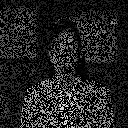
\includegraphics[width=0.8\textwidth]{Chapter7/Images/akiyo40_masked_19.png}
    \caption{Corrupted}
  \end{subfigure}
  \begin{subfigure}{0.4\textwidth}
    \centering
    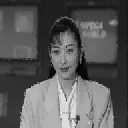
\includegraphics[width=0.8\textwidth]{Chapter7/Images/akiyo40_rec_2.png}
    \caption{Recovered}
  \end{subfigure}
  \begin{subfigure}{0.4\textwidth}
    \centering
    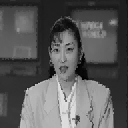
\includegraphics[width=0.8\textwidth]{Chapter7/Images/akiyo40_rec_19.png}
    \caption{Recovered}
  \end{subfigure}
  \begin{subfigure}{0.4\textwidth}
    \centering
    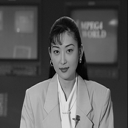
\includegraphics[width=0.8\textwidth]{Chapter7/Images/akiyo40_orig_2.png}
    \caption{Original}
  \end{subfigure}
  \begin{subfigure}{0.4\textwidth}
    \centering
    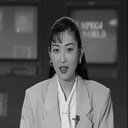
\includegraphics[width=0.8\textwidth]{Chapter7/Images/akiyo40_orig_19.png}
    \caption{Original}
  \end{subfigure}
  \caption{Reconstruction of $128\times 128\times 128$ video signal ``akiyo'' from 40\% of the measurement using the MSCE with 3 cascades. Mask decimation pattern is uniform. $\psnr = 30.02$}
\end{figure}

\begin{figure}
  \centering
  \textbf{\hspace{0.2in} Frame 32 \hspace{1.5in} Frame 52\hspace{0.5in}\vspace{0.1in}}
  \begin{subfigure}{0.4\textwidth}
    \centering
    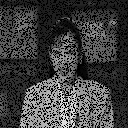
\includegraphics[width=0.9\textwidth]{Chapter7/Images/akiyo70_masked_32.png}
    \caption{Corrupted}
  \end{subfigure}
  \begin{subfigure}{0.4\textwidth}
    \centering
    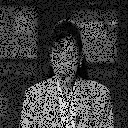
\includegraphics[width=0.9\textwidth]{Chapter7/Images/akiyo70_masked_52.png}
    \caption{Corrupted}
  \end{subfigure}
  \begin{subfigure}{0.4\textwidth}
    \centering
    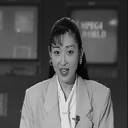
\includegraphics[width=.9\textwidth]{Chapter7/Images/akiyo70_rec_32.png}
    \caption{Recovered}
  \end{subfigure}
  \begin{subfigure}{0.4\textwidth}
    \centering
    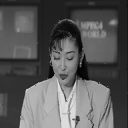
\includegraphics[width=.9\textwidth]{Chapter7/Images/akiyo70_rec_52.png}
    \caption{Recovered}
  \end{subfigure}
  \begin{subfigure}{0.4\textwidth}
    \centering
    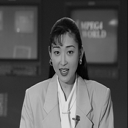
\includegraphics[width=.9\textwidth]{Chapter7/Images/akiyo70_orig_32.png}
    \caption{Original}
  \end{subfigure}
  \begin{subfigure}{0.4\textwidth}
    \centering
    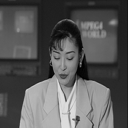
\includegraphics[width=.9\textwidth]{Chapter7/Images/akiyo70_orig_52.png}
    \caption{Original}
  \end{subfigure}
  \caption{Reconstruction of $128\times 128\times 128$ video signal ``akiyo'' from 70\% of the measurement using the MSCE with 3 cascades. Mask decimation pattern is uniform. $\psnr = 36.86$}
\end{figure}

\begin{figure}
  \centering
  \textbf{\hspace{0.2in} Frame 18 \hspace{1.5in} Frame 22\hspace{0.5in}\vspace{0.1in}}
  \begin{subfigure}{0.4\textwidth}
    \centering
    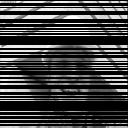
\includegraphics[width=.9\textwidth]{Chapter7/Images/foreman40_masked_18.png}
    \caption{Corrupted}
  \end{subfigure}
  \begin{subfigure}{0.4\textwidth}
    \centering
    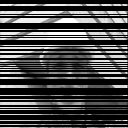
\includegraphics[width=.9\textwidth]{Chapter7/Images/foreman40_masked_22.png}
    \caption{Corrupted}
  \end{subfigure}
  \begin{subfigure}{0.4\textwidth}
    \centering
    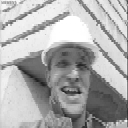
\includegraphics[width=.9\textwidth]{Chapter7/Images/foreman40_rec_18.png}
    \caption{Recovered}
  \end{subfigure}
  \begin{subfigure}{0.4\textwidth}
    \centering
    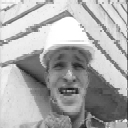
\includegraphics[width=.9\textwidth]{Chapter7/Images/foreman40_rec_22.png}
    \caption{Recovered}
  \end{subfigure}
  \begin{subfigure}{0.4\textwidth}
    \centering
    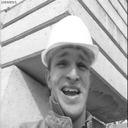
\includegraphics[width=.9\textwidth]{Chapter7/Images/foreman40_orig_18.png}
    \caption{Original}
  \end{subfigure}
  \begin{subfigure}{0.4\textwidth}
    \centering
    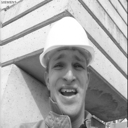
\includegraphics[width=.9\textwidth]{Chapter7/Images/foreman40_orig_22.png}
    \caption{Original}
  \end{subfigure}
  \caption{Reconstruction of $128\times 128\times 128$ video signal ``foreman'' from 40\% of the measurement using the MSCE with 3 cascades. Mask decimation pattern is: horizontal lines that are randomly generated for each frame. $\psnr = 25.50$}
\end{figure}


\begin{figure}
  \centering
  \textbf{\hspace{0.2in} Frame 18 \hspace{1.5in} Frame 22\hspace{0.5in}\vspace{0.1in}}
  \begin{subfigure}{0.4\textwidth}
    \centering
    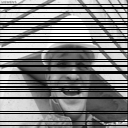
\includegraphics[width=.9\textwidth]{Chapter7/Images/foreman70_masked_18.png}
    \caption{Corrupted}
  \end{subfigure}
  \begin{subfigure}{0.4\textwidth}
    \centering
    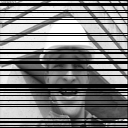
\includegraphics[width=.9\textwidth]{Chapter7/Images/foreman70_masked_22.png}
    \caption{Corrupted}
  \end{subfigure}
  \begin{subfigure}{0.4\textwidth}
    \centering
    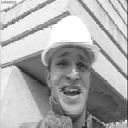
\includegraphics[width=.9\textwidth]{Chapter7/Images/foreman70_rec_18.png}
    \caption{Recovered}
  \end{subfigure}
  \begin{subfigure}{0.4\textwidth}
    \centering
    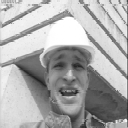
\includegraphics[width=.9\textwidth]{Chapter7/Images/foreman70_rec_22.png}
    \caption{Recovered}
  \end{subfigure}
  \begin{subfigure}{0.4\textwidth}
    \centering
    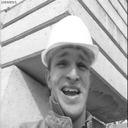
\includegraphics[width=.9\textwidth]{Chapter7/Images/foreman70_orig_18.png}
    \caption{Original}
  \end{subfigure}
  \begin{subfigure}{0.4\textwidth}
    \centering
    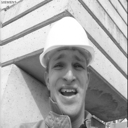
\includegraphics[width=.9\textwidth]{Chapter7/Images/foreman70_orig_22.png}
    \caption{Original}
  \end{subfigure}
  \caption{Reconstruction of $128\times 128\times 128$ video signal ``foreman'' from 70\% of the measurement using the MSCE with 3 cascades. Mask decimation pattern is: horizontal lines that are randomly generated for each frame. $\psnr = 30.32$}
\end{figure}

\begin{figure}
  \centering
  \textbf{\hspace{0.2in} Frame 11 \hspace{1.5in} Frame 12\hspace{0.5in}\vspace{0.1in}}
  \begin{subfigure}{0.4\textwidth}
    \centering
    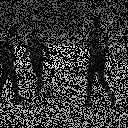
\includegraphics[width=.9\textwidth]{Chapter7/Images/soccer40_masked_11.png}
    \caption{Corrupted}
  \end{subfigure}
  \begin{subfigure}{0.4\textwidth}
    \centering
    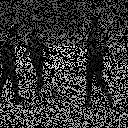
\includegraphics[width=.9\textwidth]{Chapter7/Images/soccer40_masked_12.png}
    \caption{Corrupted}
  \end{subfigure}
  \begin{subfigure}{0.4\textwidth}
    \centering
    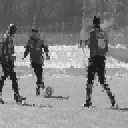
\includegraphics[width=.9\textwidth]{Chapter7/Images/soccer40_rec_11.png}
    \caption{Recovered}
  \end{subfigure}
  \begin{subfigure}{0.4\textwidth}
    \centering
    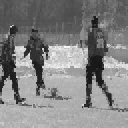
\includegraphics[width=.9\textwidth]{Chapter7/Images/soccer40_rec_12.png}
    \caption{Recovered}
  \end{subfigure}
  \begin{subfigure}{0.4\textwidth}
    \centering
    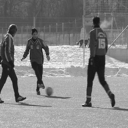
\includegraphics[width=.9\textwidth]{Chapter7/Images/soccer40_orig_11.png}
    \caption{Original}
  \end{subfigure}
  \begin{subfigure}{0.4\textwidth}
    \centering
    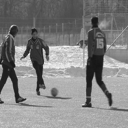
\includegraphics[width=.9\textwidth]{Chapter7/Images/soccer40_orig_12.png}
    \caption{Original}
  \end{subfigure}
  \caption{Reconstruction of $128\times 128\times 128$ video signal ``soccer'' from 40\% of the measurement using the MSCE with 3 cascades. Mask decimation pattern is: missing pixels that are constant across the frames. $\psnr = 24.84$}
\end{figure}



\begin{figure}
  \centering
  \textbf{\hspace{0.2in} Frame 11 \hspace{1.5in} Frame 12\hspace{0.5in}\vspace{0.1in}}
  \begin{subfigure}{0.4\textwidth}
    \centering
    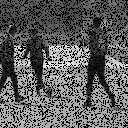
\includegraphics[width=.9\textwidth]{Chapter7/Images/soccer70_masked_11.png}
    \caption{Corrupted}
  \end{subfigure}
  \begin{subfigure}{0.4\textwidth}
    \centering
    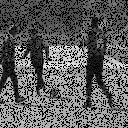
\includegraphics[width=.9\textwidth]{Chapter7/Images/soccer70_masked_12.png}
    \caption{Corrupted}
  \end{subfigure}
  \begin{subfigure}{0.4\textwidth}
    \centering
    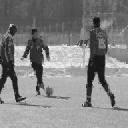
\includegraphics[width=.9\textwidth]{Chapter7/Images/soccer70_rec_11.png}
    \caption{Recovered}
  \end{subfigure}
  \begin{subfigure}{0.4\textwidth}
    \centering
    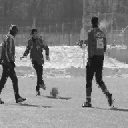
\includegraphics[width=.9\textwidth]{Chapter7/Images/soccer70_rec_12.png}
    \caption{Recovered}
  \end{subfigure}
  \begin{subfigure}{0.4\textwidth}
    \centering
    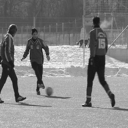
\includegraphics[width=.9\textwidth]{Chapter7/Images/soccer70_orig_11.png}
    \caption{Original}
  \end{subfigure}
  \begin{subfigure}{0.4\textwidth}
    \centering
    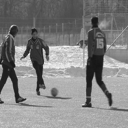
\includegraphics[width=.9\textwidth]{Chapter7/Images/soccer70_orig_12.png}
    \caption{Original}
  \end{subfigure}
  \caption{Reconstruction of $128\times 128\times 128$ video signal ``soccer'' from 70\% of the measurement using the MSCE with 3 cascades. Mask decimation pattern is: missing pixels that are constant across the frames. $\psnr = 29.35$}
\end{figure}

\begin{figure}
  \centering
  \textbf{\hspace{0.5in} Frame 21 \hspace{1.5in} Frame 151\hspace{0.5in}\vspace{0.2in}}
  \begin{subfigure}{0.4\textwidth}
    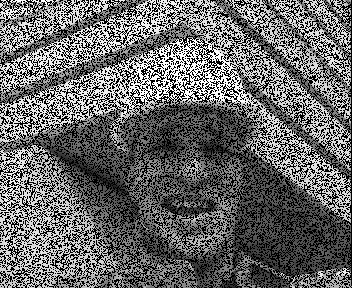
\includegraphics[width=\textwidth]{Chapter5/Images/foreman_masked_21.png}
    \caption{Corrupted}
  \end{subfigure}
  \begin{subfigure}{0.4\textwidth}
    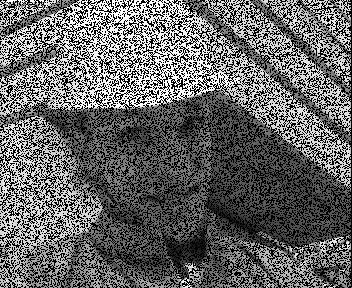
\includegraphics[width=\textwidth]{Chapter5/Images/foreman_masked_151.png}
    \caption{Corrupted}
  \end{subfigure}
  \begin{subfigure}{0.4\textwidth}
    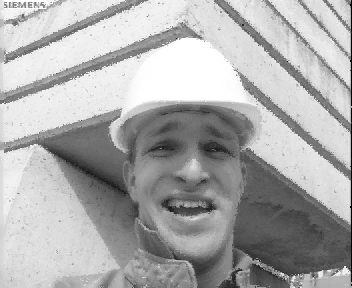
\includegraphics[width=\textwidth]{Chapter5/Images/foreman_rec_21.png}
    \caption{Recovered}
  \end{subfigure}
  \begin{subfigure}{0.4\textwidth}
    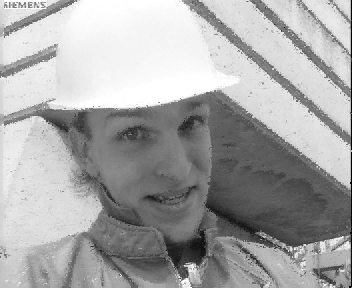
\includegraphics[width=\textwidth]{Chapter5/Images/foreman_rec_151.png}
    \caption{Recovered}
  \end{subfigure}
  \begin{subfigure}{0.4\textwidth}
    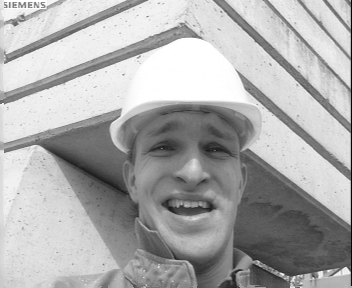
\includegraphics[width=\textwidth]{Chapter5/Images/foreman_orig_21.png}
    \caption{Original}
  \end{subfigure}
  \begin{subfigure}{0.4\textwidth}
    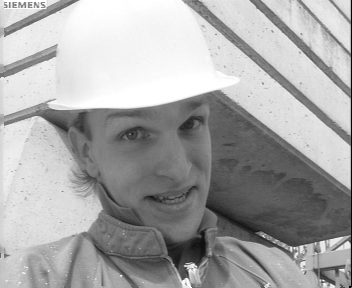
\includegraphics[width=\textwidth]{Chapter5/Images/foreman_orig_151.png}
    \caption{Original}
  \end{subfigure}
  \caption[Example output of our video interpolator]{Example of a masked video signal, where only 60\% of the pixel values are known (a-b). 
    Reconstruction via the MSCE Algorithm using 2 cascades (PSNR: 28.6) (c-d).
    Original video (e-f).}
  \label{fig:foreman_masked}
\end{figure}
